%%%%%
%%%%% File name  : hw1_report.tex
%%%%% Author     : Yueh-Chou Lee
%%%%% Date       : March 26, 2020
%%%%%
%%
%%%
\documentclass[a4paper,11pt]{article}
\usepackage[top=2cm,bottom=2cm,outer=2cm,inner=2cm]{geometry}
\usepackage[utf8]{inputenc}
\usepackage[T1]{fontenc}
\usepackage{fontspec}
\usepackage{xeCJK}
\usepackage{amsfonts}
\usepackage{amsmath}
\usepackage{graphicx}
\usepackage{subfigure}
\usepackage{setspace}
\usepackage[explicit]{titlesec}
\usepackage{titlesec}
\usepackage{bibentry}
\usepackage[nottoc,numbib]{tocbibind} 
\usepackage{filecontents}
\usepackage{color}
\renewcommand{\baselinestretch}{2}
\setCJKmainfont{標楷體}


\title{Machine Learning Homework 1 Report}
\author{R06221012\hspace{0.2cm}數學所\hspace{0.2cm}李岳洲}
\date{March 26, 2020}

\begin{document}

\maketitle

\begin{enumerate}
	\item \textit{\textbf{使用四種不同的 learning rate 進行 training (其他參數需一致),作圖並討論其收斂過程。}}\\

	For the train or validation set, the convergence rate of different learning rates at loss is $10 > 1 > 100 > 0.1$ (Figure 1). This experiment uses \textbf{Aadagrad} as the weight update method. Aadagrad method is to slow down the gradient descent update step as the number of iterations increases, so the smaller the learning rate will cause the smaller update step of gradient descent. In addition, the initial learning rate $= 10$ is the best choice from this experiment (compare to $0.1, 1, 100$). However, by using the larger learning rate, the loss will eventually converge to the global minimum, and if the learning rate is too small, the loss will not converge the global minimum (only stop at the local minimum).\\

	\begin{figure}[htp]
	    \begin{center}
	    	\subfigure[Training loss]{
	    		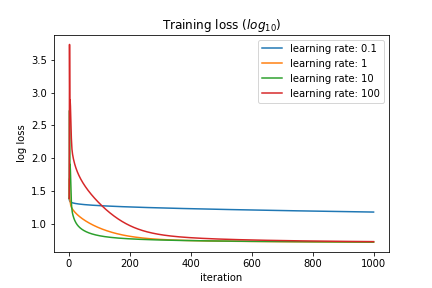
\includegraphics[scale=0.5]{training_loss.png}
	    	}
	    	\quad
	    	\subfigure[Validation loss]{
	    		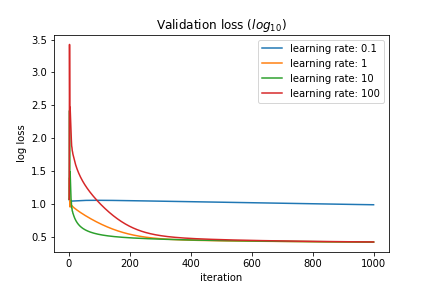
\includegraphics[scale=0.5]{validation_loss.png}
	    	}
	    	\caption{Loss}
	    \end{center}
	\end{figure}


% \newpage

	\item \textit{\textbf{比較取前 5 hrs 和前 9 hrs 的資料(5*18 + 1 v.s 9*18 + 1)在 validation set 上預測的結果,並說明造成的可能原因。}}

	Using all features during 9 hours will be better than using all features during 5 hours. Using features during only 5 hours will fast converge (Figure 2) but its convergent loss is worse than using features during 9 hours (Table 1). The reasons might be (1) more information will cause slower convergence and (2) training with more than one information will have the opportunity to lead to lower loss.\\

	\begin{figure}[htp]
	    \begin{center}
    		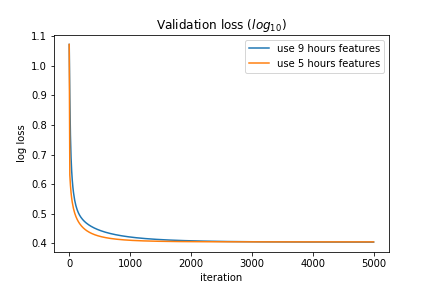
\includegraphics[scale=0.5]{loss_9hr_vs_5hr.png}
	    	\caption{Loss with using 9 hours and 5 hours features}
	    \end{center}
	\end{figure}
.\newline
	\begin{table}[htp]
		\begin{center}
			\begin{tabular}{ | c | c | }
			  	\hline
		  		9 hours features & 5 hours features\\[0.5ex] 
		  		\hline \hline
		  		2.53420 & 2.53849\\[0.2ex]
		  		\hline
			\end{tabular}
			\caption{Minimum of validation loss}
		\end{center}
	\end{table}

	\item \textit{\textbf{比較只取前 9 hrs 的 PM2.5 和取所有前 9 hrs 的 features(9*1 + 1 vs. 9*18 + 1)在 validation set上預測的結果,並說明造成的可能原因。}}

	Using all features will be better than only one feature (PM 2.5). Using only one feature will fast converge (Figure 3) but its convergent loss is worse than using all features (Table 2). The reasons might be (1) using only single information (use PM 2.5 to predict PM 2.5) will let the loss quickly converge to the local minimum and (2) training with more than one feature (PM 2.5) will extract more information to predict the result so that the prediction will be more accurate.\\

	\begin{figure}[htp]
	    \begin{center}
    		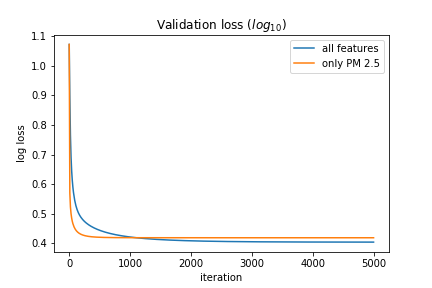
\includegraphics[scale=0.5]{loss_pm25_vs_all.png}
	    	\caption{Loss with using only PM 2.5 and all features}
	    \end{center}
	\end{figure}

	\begin{table}[htp]
		\begin{center}
			\begin{tabular}{ | c | c | }
			  	\hline
		  		all features & only PM 2.5\\[0.5ex] 
		  		\hline \hline
		  		2.53420 & 2.62185\\[0.2ex]
		  		\hline
			\end{tabular}
			\caption{Minimum of validation loss}
		\end{center}
	\end{table}

	\item \textit{\textbf{請說明你超越 baseline 的 model (最後選擇在Kaggle上提交的) 是如何實作的。}}

	\begin{enumerate}
		\item [\textit{Step 1.}] \textit{Data Preprocessing}
			\begin{enumerate}
				\item [a.] Replace 'NR' to the value $0.0$:\\
				'NR' in the row of RAINFALL isn't a numerical value so we cannot directly use non-numerical value to construct the multivariate linear regression.

				\item [b.] Not normalize our dataset!\\
			\end{enumerate}

		\item [\textit{Step 2.}] \textit{Features Extraction}

		\textbf{Pearson Correlation Coefficient:}

		We collect all 18 features into the $18 \times N$ matrix and calculate the \textbf{Pearson Correlation Coefficient} between all features and PM 2.5. Then we extract 7 features that are highly or moderately correlated $(abs(\rho) \geq 0.3)$.\\

		\begin{table}[htp]
			\begin{center}
				\begin{tabular}{ | c | c | c | }
				  	\hline
			  		Highly Correlated &  Moderately Correlated & Low Correlated\\[0.5ex] 
			  		\hline \hline
			  		$abs(\rho) \geq 0.7 $& $0.7 > abs(\rho) \geq 0.3$ & $0.3 > abs(\rho) > 0$\\[0.2ex]
			  		\hline
				\end{tabular}
				\caption{Correlation coefficient rank}
			\end{center}
		\end{table}


		\item [\textit{Step 3.}] \textit{Train}

		\textbf{Setting:}
			\begin{enumerate}
				\item [a.] Loss function: RMSE
					$$RMSE = \sqrt{\frac{\sum_{i = 1}^N {y_{\text{pred}}}_i - {y_{\text{act}}}_i}{N}}$$

				\item [b.] Update of weights: Adagrad
					$$\text{\textbf{Adagrad:}}
					\quad w^{t+1} \leftarrow w^t - \frac{\eta}{\sum_{i = 0}^t (\text{gradient}^i)^2}\,\text{gradient}^t$$

				\item [c.] Learning rate: 4.15

				\item [d.] Maximum iteration: 100000

				\item [e.] Early stopping iteration: 1000, stop training by judging the validation loss.\\

			\end{enumerate}

		\item [\textit{Step 4.}] \textit{Round}

		Let $Y_{\text{pred}} = [{y_{\text{pred}}}_1,\,{y_{\text{pred}}}_2,\,{y_{\text{pred}}}_3, \cdots, {y_{\text{pred}}}_i, \cdots ]$ be our first prediction\\and $Y_{\text{round}} = [{y_{\text{round}}}_1,\,{y_{\text{round}}}_2,\,{y_{\text{round}}}_3, \cdots, {y_{\text{round}}}_i, \cdots ]$ be our round result. Then we get the final prediction by using the following condition.

			$${y_{\text{round}}}_i =
			\left\{\begin{matrix}
				&round({y_{\text{pred}}}_i),
				&\quad \text{if $abs({y_{\text{pred}}}_i - {y_{\text{round}}}_i) < 0.1$}\\
				&{y_{\text{pred}}}_i,
				&\quad \text{otherwise}
			\end{matrix}\right.$$\\

		\item [\textit{Result}].

		\begin{table}[htp]
			\begin{center}
				\begin{tabular}{| c | c | c | c | c | }
				  	\hline
			  		& Simple baseline & Simple model & Strong baseline & Best model\\[0.5ex] 
			  		\hline \hline
			  		Loss & 6.55912 & 5.65410 & 5.55972 & 5.40732\\[0.2ex]
			  		\hline
				\end{tabular}
				\caption{Kaggle's public test set loss}
			\end{center}
		\end{table}
	\end{enumerate}
\end{enumerate}


\end{document}





